\chapter{Introduction}
\label{ch1}

%%%%% https://cerncourier.com/a/pushing-the-precision-frontier/
% https://home.cern/news/news/physics/why-precision-luminosity-measurements-matter
Particle physics is the branch of physics that studies the fundamental components of matter and the interactions that govern their behavior. It is based on the Standard Model, a theoretical framework that classifies elementary particles into fermions, which make up matter, and bosons, which mediate the fundamental forces (except gravity, which is not yet incorporated into this model). To investigate these particles and their interactions, high-energy particle accelerators are used to generate collisions that allow scientists to measure particle properties and study fundamental phenomena.

This introduction provides a general overview of elementary particles, particle colliders, and the measurement of their properties, establishing the groundwork for studying theoretical and experimental models in particle physics. It highlights key concepts and definitions essential for understanding this project.

\section{Particle Physics and The Standard Model}


Matter and its fundamental interactions are governed by 17 elementary particles that make up the \textbf{Standard Model} of particle physics. These particles are divided into two main groups: fermions, which have a spin of \( \frac{1}{2} \), and bosons, which have an integer spin. Matter is primarily composed of fermions, which include twelve fundamental particles classified into two types: leptons and quarks. These particles are organized into three generations, with each successive generation having a greater mass than its corresponding particle in the previous generation \cite{thomson_2013}.\\

The group of six leptons includes three charged particles: the electron (\(e^-\)), the muon (\(\mu^-\)), and the tau (\(\tau^-\)), along with their corresponding neutrinos: the electron neutrino (\(\nu_e\)), the muon neutrino (\(\nu_\mu\)), and the tau neutrino (\(\nu_\tau\)). On the other hand, quarks are only found in hadrons. The group of six quarks consists of: the up quark (\(u\)), the down quark (\(d\)), the charm quark (\(c\)), the strange quark (\(s\)), the top quark (\(t\)), and the bottom quark (\(b\)) \cite{griff,thomson_2013}. The properties of these twelve particles are summarized in Table \ref{tab:table1}.


\begin{table}[h!]
	\begin{center}
%\centering
	\caption[The twelve fundamental fermions and their properties]{Classification and properties of the twelve fundamental Fermions divided between Quarks and Leptons\cite{thomson_2013}.}
		\label{tab:table1}
		\begin{tabular}{lllrcllrc}
                                                                                & \multicolumn{4}{c}{\textbf{Leptons}}                                                                     & \multicolumn{4}{c}{\textbf{Quarks}}                                                \\ 
%\cline{2-9}
 \midrule[1.1pt]
                            \multicolumn{1}{c}{Generation }& \multicolumn{2}{c}{Particle } & \multicolumn{1}{c}{\textit{Q}} & mass/GeV                          & \multicolumn{2}{c}{Particle} & \multicolumn{1}{c}{\textit{Q}} & mass/GeV  \\ 
\hline
\multirow{2}{*}{\begin{tabular}[c]{@{}l@{}}First\end{tabular}}  & electron & ($e$\textsuperscript{-})                 & -1                             & 0.0005                            & down    & ($d$)                & -1/3                           & 0.003     \\
                                                                                & $e$-neutrino & ($\nu_{e}$)                 & 0                              & \textless{}10\textsuperscript{-9} & up      & ($u$)                & +2/3                           & 0.005     \\
\multirow{2}{*}{\begin{tabular}[c]{@{}l@{}}Second\end{tabular}} & muon     & (${\mu}$\textsuperscript{-})                 & -1                             & 0.106                             & strange & ($s$)                & -1/3                           & 0.1       \\
                                                                                & $\mu$-neutrino & ($\nu_{\mu}$)                 & 0                              & \textless{}10\textsuperscript{-9} & charm   & ($c$)                & +2/3                           & 1.3       \\
\multirow{2}{*}{\begin{tabular}[c]{@{}l@{}}Third\end{tabular}} & tau      & ({$\tau}$\textsuperscript{-})                 & -1                             & 1.78                              & bottom  & ($b$)                & -1/3                           & 4.5       \\
                                                                                & $\tau$-neutrino & ($\nu_{\tau}$)                 & 0                              & \textless{}10\textsuperscript{-9} & top     &($t$)                & +2/3                           & 174      
\end{tabular}
	\end{center}
		\end{table}

Bosons act as mediators of interactions between fermions by exchanging particles known as gauge bosons. The electromagnetic force is mediated by the photon (\(\gamma\)), which interacts with charged particles such as electrons (\(e^-\)) and protons (\(p\)). The weak force is mediated by the \(W^{\pm}\) and \(Z^{0}\) bosons, interacting with all leptons and quarks, facilitating processes like beta decay in nuclei. The strong force, responsible for holding quarks together within protons and neutrons, is carried by gluons (\(g\)), and it only interacts with quarks and gluons themselves, forming the strong interaction that binds hadrons together. Additionally, the Higgs boson, a scalar boson, plays a crucial role in providing mass to all fundamental particles through the Higgs mechanism, which affects both fermions and bosons \cite{thomson_2013}. Table \ref{tab:table2} provides a comprehensive overview of the forces experienced by fermions.


\begin{table}[h!]
  \begin{center}
    \caption[Force experienced by the fermions]{Force experienced by the fermions \cite{thomson_2013}.}
    \label{tab:table2}
    \begin{tabular}{l c c c c}
    &    &  \textbf{Electromagnetic} & \textbf{Weak} & \textbf{Strong}\\
      \midrule[1.1pt]
      \multirow{2}{*}{Leptons} & ${e}$\textsuperscript{-} \hspace{0.3cm}  ${\mu}$\textsuperscript{-} \hspace{0.3cm} ${\tau}$\textsuperscript{-} & \checkmark & \checkmark & \\ % <-- Combining 2 rows with arbitrary with (*) and content 12
      & $ \nu_{e} $ \hspace{0.3cm}  $\nu_{\mu}$ \hspace{0.3cm} $\nu_{\tau}$  &  & \checkmark\\ % <-- Content of first column omitted.
      \hline
      \multirow{2}{*}{Quarks} & $u$ \hspace{0.5cm}  $c$\hspace{0.5cm} $t$ & \checkmark & \checkmark& \checkmark\\
      & $d$ \hspace{0.5cm}  $s$\hspace{0.5cm} $b$ & \checkmark & \checkmark & \checkmark\\

    \end{tabular}
  \end{center}
\end{table}

So far, the Standard Model (SM) of particle physics is the most precise and successful theoretical model for describing experimental data available to date. This model provides a detailed explanation of the fundamental interactions between elementary particles. However, most of this data comes from experiments conducted at particle colliders, as these devices allow the production and study of particles through high-energy collisions, making it possible to observe phenomena that cannot be studied otherwise. Despite its success, the Standard Model still has limitations and cannot explain some aspects of the universe, such as gravity, dark matter, and dark energy.


\section{Luminosity}


Particle colliders are powerful scientific instruments used to produce, accelerate, and collide beams of particles at relativistic speeds, enabling scientists to explore the fundamental properties of matter and the universe. These experiments function as powerful microscopes that allow researchers to study subatomic particles such as electrons, protons, neutrons, neutrinos, and quarks. They areevaluated based on two important measures, which are the available center of mass energy and the rate at which particles collide (luminosity).

When the particles in the beams have equal energy and opposite momentum (equal mass), the experiment occurs in the center-of-mass (CM) frame. This allows for the entire energy delivered by the accelerator to be utilized in generating high-mass particles \cite{undergraduate_accelerators_chapter}. In particle physics, the Lorentz invariant quantity $s$ represents the square of the total incoming energy and is defined as:

\begin{equation}
s = \left ( \sum_{i = 1,2}^{}E_{i} \right )^{2}-\left ( \sum_{i = 1,2}^{}p_{i} \right )^{2}c^{2}
\end{equation}

Where  \textbf{$p$} and $E$ are the momenta and the energy of each incoming particle respectively.In the center-of-mass (CM) frame, where the momenta of the particles are equal and opposite, the second term in the equation for the Lorentz invariant quantity ($s$) disappears, leaving only $s = 4E^2$.\\

The second important parameter used to evaluate the performance of colliders is luminosity, which measures the accelerator's ability to produce the necessary number of interactions. It is determined by the proportionality factor between the quantum mechanical probability for the interaction (known as the cross section) and the number of events for a specific physics process per second ($R$) \cite{ref_lib_vol3}.\\

When two beams cross in a particle accelerator, a variety of different processes can occur and  the cross section of a given process depends on the type and energy of the colliding particles.
At the Large Hadron Collider (LHC), certain particles such as  $W^{\pm}$ and $Z^{0}$ bosons have large cross sections , making their observation more frequent, while the production of a Higgs boson has a much lower cross section, making it more difficult to produce \cite{thomson_2013}.\\

To illustrate this concept more clearly, let's consider a simple scenario where a beam of particles of type $a$ passes through a region of space that contains particles of type $b$. The interaction rate between the two types of particles depends on the number of particles per unit volume of type $b$, denoted as $n_{b}$, and the flux of the incident particles, denoted as $\phi_{a}$. The rate of interaction per target particle of type $b$ can be expressed as follows:

\begin{equation*}
  r_{b}=\sigma \phi_{a}
\end{equation*}

Figure \ref{cross_section}(a) shows an illustration of this concept, where an incident particle of type $a$ moves with velocity $v_{a}$ through a region of area $A$ that contains target particles of type $b$ with velocity $v_{b}$ moving in the opposite direction \cite{thomson_2013}.

\begin{center}
  \begin{figure}[h!]
    \centering
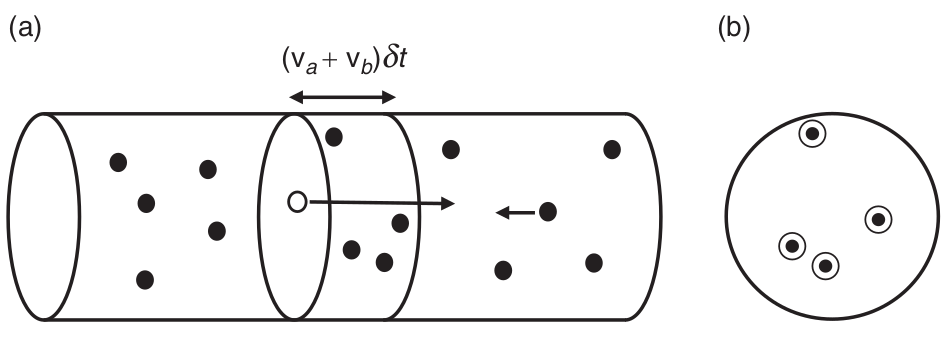
\includegraphics[scale=.35]{Chapter1/cross_section.png} 
 \caption[Cross section illustration]{Left hand (a): single incident particle of type $a$ traversing a region containing particles of type $b$. Right-hand plot (b): projected view of the region traversed by the incident particle in time $\delta t$.}
    \label{cross_section}
  \end{figure}
\end{center}

In particle physics experiments, the number of useful interactions (or events) is a crucial, the capability of a particle accelerator to produce such interactions is quantified by a parameter known as the instantaneous luminosity, denoted as $\mathcal{L}_{\text{inst}}$. The significance of luminosity lies in its direct relationship with the production rate of particles of interest. Specifically, the rate at which a particular process occurs is proportional to the product of the luminosity and the corresponding cross section. As such, luminosity directly impacts the ability to observe rare events. Furthermore, achieving precise measurements of particle properties often requires a large number of collisions to ensure sufficient statistical significance.

The event rate $R$ for a given process is defined as the product of the instantaneous luminosity and the process cross section $\sigma_p$~\cite{concept_of_luminosity}:

\begin{equation}
R = \mathcal{L}_{\text{inst}} \cdot \sigma_p
\label{eq.lumi}
\end{equation}

Here, luminosity is expressed in units of $cm^{-2}s^{-1}$.

The cross section of the process that produces the particle is a measure of the probability that a given interaction will occur. It is typically a very small quantity, on the order of picobarns ($10^{-36}~\text{cm}^2$). To achieve high luminosity, particle accelerators employ various techniques to increase the number of particles in the beams and to focus them into a small cross-sectional area. This is accomplished through the use of superconducting magnets, which guide and confine the particles to a narrow path. Additionally, radio frequency (RF) cavities are used to accelerate the particles to higher energies, thereby increasing the frequency of bunch crossings and enhancing the overall collision rate.


In high-energy particle accelerators, such as the Large Hadron Collider (LHC) at CERN, integrated luminosity is a key quantity that measures the total number of collisions per unit area accumulated during an experiment. It quantifies the total amount of data collected and is crucial for evaluating the performance of the accelerator. Integrated luminosity is defined as~\cite{concept_of_luminosity}:

\begin{equation}
  \mathcal{L}_{\text{int}} = \int_{0}^{T} \mathcal{L}_{\text{inst}}(t')\,dt'
\end{equation}

Here, $\mathcal{L}_{\text{inst}}$ is evaluated over the duration $T$ of the data-taking period (excluding possible dead time), as its intensity typically decreases over time due to the reduction in the number of protons during the fill.

Precisely understanding luminosity is really important for physics analyses like finding new particles, measuring known particle properties, or detecting rare processes. The accuracy of our physics measurements is mainly affected by uncertainties in luminosity. If we can increase the precision of luminosity measurements, then physicists will have a better understanding of their observations and be able to explore parts of physics that we don't currently know about \cite{luminosity_importance}.

An example of this can be seen in Fig. \ref{lumi_incertainty}, which illustrates the production of $W$ and $Z$ bosons in the large hadron collider. In this figure, the inner error bars represent the experimental uncertainties, while the outer error bars encompass the uncertainties in the theoretical predictions. Additionally, the shaded box indicates the uncertainties in the luminosity measurement, which is bigger that statistical and other systematics uncertainties \cite{lumi_uncertainties}.

\begin{center}
  \begin{figure}[h]
    \centering
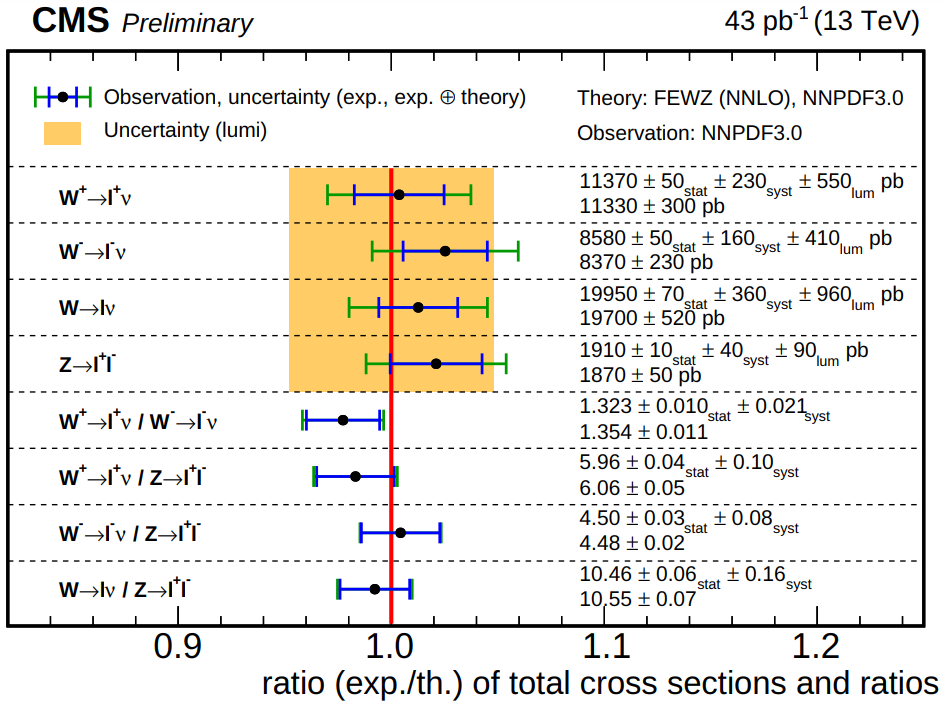
\includegraphics[scale=.28]{Chapter1/lumi_uncertainty.png} 
 \caption[Luminosity uncertainty in a process]{Production of $W^+$, $W^-$, $W$ and $Z$ bosons and their theoretical predictions. The shaded box indicates the uncertainties in the luminosity measurement, showing that is bigger than the experimental (blue bars) and heoretical (green bars) uncertainties. The measurements and theoretical predictions values are on the right}
    \label{lumi_incertainty}
  \end{figure}
\end{center}


\section{The Large Hadron Collider}
 
The Large Hadron Collider (LHC) is the world's biggest and most potent particle accelerator. It became operational on 10th September 2008 and is the most recent addition to CERN's accelerator complex. The LHC consists of a 27-kilometer ring that contains superconducting magnets, and various structures are used to accelerate particles as they move along the ring. Inside the accelerator, two particle beams travel at almost the speed of light until they collide. The beams move in opposite directions in separate beam pipes, which are kept at an ultra-high vacuum.\\ 

Superconducting electromagnets generate a powerful magnetic field that guides the particle beams around the accelerator ring. These magnets are made up of coils of a unique electric cable that functions in a superconducting state. In this state, the cable can conduct electricity with zero resistance or energy loss. The accelerator uses a variety of magnets, including 1232 dipole magnets that are 15 metres in length and bend the beams, and 392 quadrupole magnets that are 5-7 metres long and focus the beams. Just before the collision, a different type of magnet is employed to "squeeze" the particles together, increasing the likelihood of collisions. To keep these magnets in the superconducting state, they must be cooled to a temperature as low as -271.3°C \cite{LHC}.\\

The process of generating proton beams for the LHC is a complex and multi-stage procedure. Initially, hydrogen is ionized to create protons, which are then accelerated in bunches up to 50 MeV in the Linear Accelerator 2 (LINAC2). The proton bunches are then routed through three circular accelerators: the Booster, the Proton Synchrotron (PS), and the Super Proton Synchrotron (SPS). These accelerators gradually increase the energy levels of the proton bunches to 1.4 GeV, 26 GeV, and 450 GeV, respectively \cite{lhc_complex}. Once these pre-acceleration stages are completed, the proton bunches are injected into the LHC ring where they are further accelerated to achieve energies of up to 7 TeV per bunch while circulating in opposite directions. This entire process constitutes a single LHC fill and typically involves $10^{14}$ protons that are grouped into bunches to form the proton beam. The complete CERN accelerator complex is illustrated in Figure \ref{lhc_com}.

\begin{center}
  \begin{figure}[h]
    \centering
    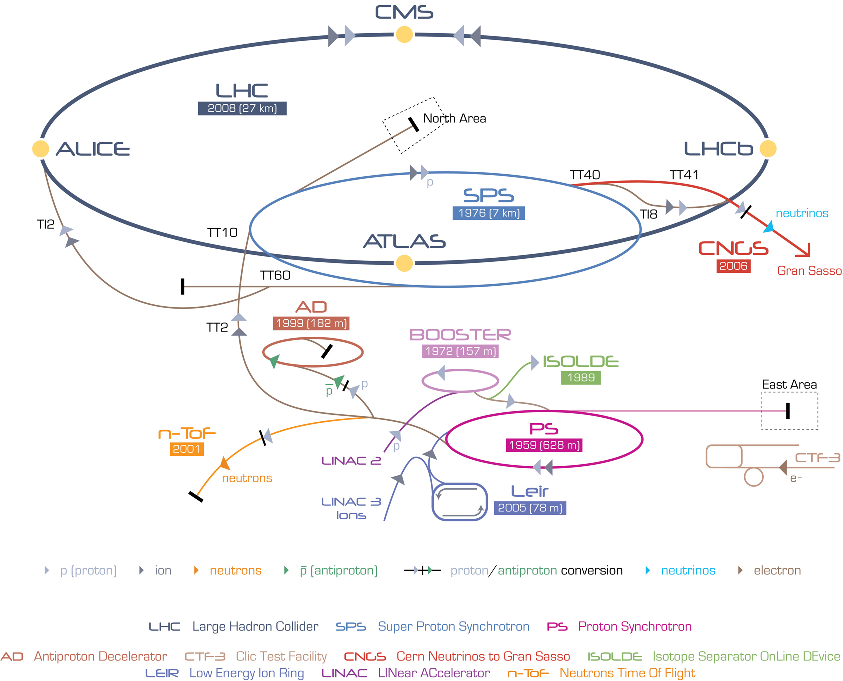
\includegraphics[scale=.45]{Chapter1/lhc_complex_fig.png}
    \caption[LHC Complex]{Diagram of the LCH complex \cite{lhc_complex}.}
    \label{lhc_com}
  \end{figure}
\end{center}

The CERN Control Centre serves as the central hub responsible for managing all controls, services, and technical infrastructure of the LHC. It directs the proton beams to collide at four distinct locations along the accelerator ring, corresponding to the positions of four particle detectors: CMS and ATLAS, which are general-purpose detectors designed to explore a broad range of Standard Model (SM) and Beyond SM (BSM) physics, while ALICE and LHCb are specialized detectors that focus on studying specific phenomena.

\section{Current Luminosity precision for LHC Run 2}

Since its inception in 2010 the LHC has undergone three runs and two lengthy shutdowns for maintenance and upgrades. 
Run1 began in 2010 with proton-proton collisions at a center-of-mass energy of $\sqrt{s}=\text{7 TeV}$ and concluded in 2012 at  $\sqrt{s}=\text{8 TeV}$. Run 2, which took place at $\sqrt{s}=\text{13 TeV}$, was divided into two stages; the first  occurred from 2015 to 2016.\\

The second stage (2017–2018) had preliminary results published in the Public Analysis Summaries for 2017 and 2018 \cite{pas_17,pas_18}. However, the desired uncertainty values were not achieved.
Efforts are currently underway to further improve the precision of these measurements and present them in a final publication. This project is primarily focused on contributing to this publication by analyzing the PCC luminometer and refining the uncertainty, aiming to achieve values of approximately 1\%.\\

The integrated luminosity for Run 2, along with its corresponding uncertainty values, is presented in Table \ref{lumi_values}. These luminosity values account for the period from the start of stable beams until the beam is dumped by the LHC. Additionally, Figure \ref{lumi_per_year_int} provides a visualization of the delivered luminosity over time for each year, as measured by CMS.

% for both years.
% ref. TDR Bril para los 390
%separar por lumpas , poner  referencia, poner periodo en vez de Run
%-  en incertidumbre  no conocida, dejar solamente 2022
\begin{table}[h!]
    \begin{center}
    \caption[Integrated luminosity values delivered by Run 2]{Integrated luminosity values delivered by Run 2 (precision values ​​for the years 2017 and 2018 show preliminary results)}
	\label{lumi_values}
\begin{tabular}{cccc}
\textbf{Period} & \textbf{Energy $\sqrt{s}$} & \begin{tabular}[c]{@{}c@{}}\textbf{Integrated}\\\textbf{Luminosity}\end{tabular} & \textbf{Precision}    \\ 
\toprule
Run 1(2010-2012) \cite{PCC_PAS_12_001} & 8 TeV                   & $30 fb^{-1}$                         & 2.2\%                 \\
Run 2(2015-2016) \cite{lumi_precise_2015_2016} & 13 TeV   & $45.9 fb^{-1}$                     & 1.6\%-1.2\%                \\
Run 2(2017) \cite{pas_17} & 13 TeV                                                   & $49.8 fb^{-1}$                     & 2.3\%                 \\
Run 2(2018) \cite{pas_18} & 13 TeV                                                  & $67.9 fb^{-1}$                      & 2.5\%                 \\
\end{tabular}
    \end{center}
\end{table}


%%%%%%%%%%%%%%%%%%%%%%%%%%%%%%%%%%%%%%%%%%%%%%

  \begin{center}
  \begin{figure}[ht]
    \centering
    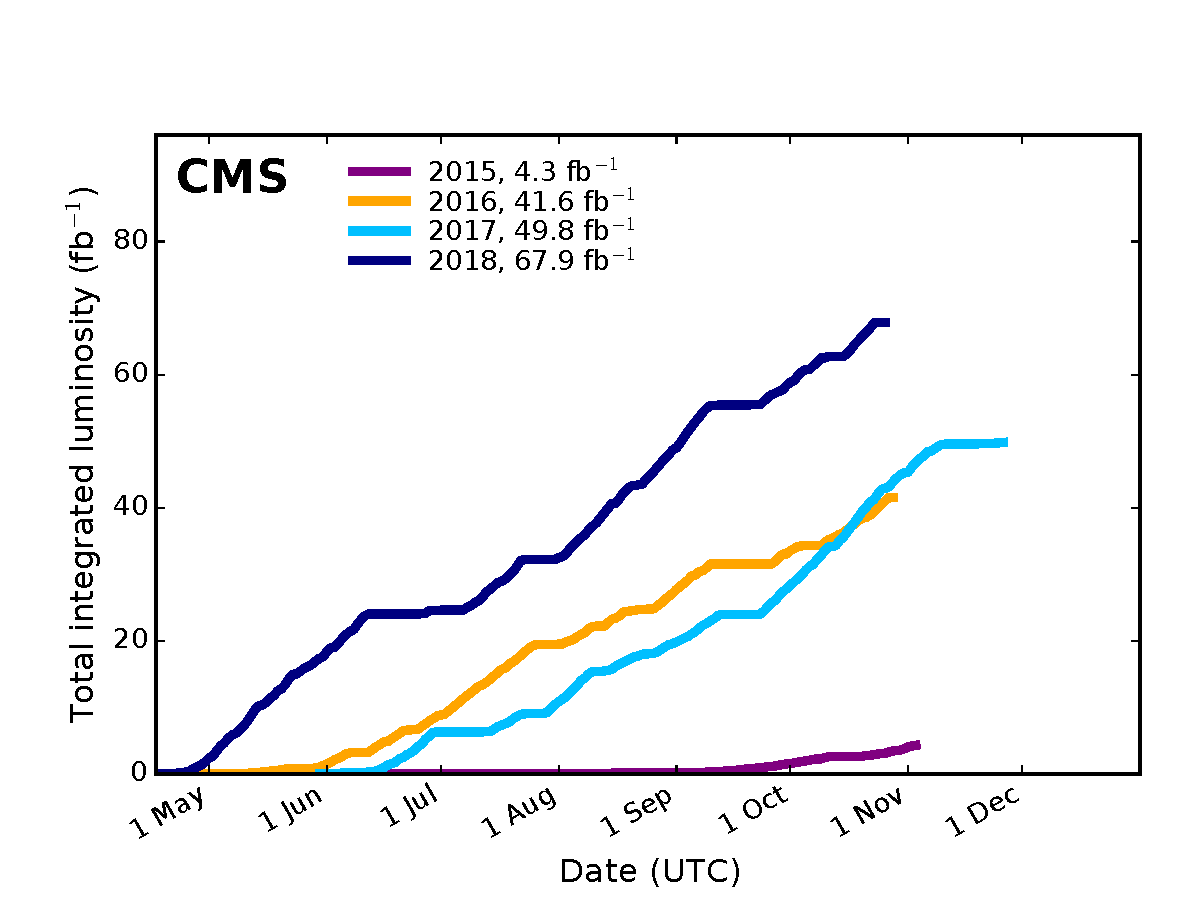
\includegraphics[scale=.55]{Chapter1/int_lumi_cumulative_pp_2_run2.pdf}
    \caption[Delivered integrated luminosity per year]{Delivered luminosity versus time for Run-1 (2010-2012) and Run-2 (2015-2018) and Run-3 that is still ongoing . Cumulative luminosity versus day delivered to CMS during stable beams for pp collisions at nominal center-of-mass energy.  \cite{wikicern}.}
    \label{lumi_per_year_int}
  \end{figure}
    \end{center}
    
